\documentclass{llncs}
\usepackage[english]{babel}
\usepackage[T1]{fontenc}
\usepackage[utf8]{inputenc}
\usepackage{graphicx}
\usepackage{color}
\usepackage{comment}
\usepackage{amsmath}

\pagestyle{plain}
\newcommand{\todo}[1]{{\color{red}TODO:~#1}}

\title{The Catchy Title (1000 Readers)}
\author{Your names}
\institute{Hasso Plattner Institute, Potsdam, Germany}

\begin{document}

\maketitle

\begin{abstract}
%!TEX root = ../paper.tex
%100 readers 4-6 Sentences

% 4 sentences:
% State the problem
% Say why it’s an interesting problem
% Say what your solution achieves
% Say what follows from your solution
\end{abstract}

%!TEX root = ../paper.tex

\section{Introduction}
\label{sec:introduction}

Due to the immense growth of the internet and the blogosphere, users have an overwhelming amount of potential reading material available.
Since maintaining a blog requires very little technical knowledge, nearly anyone can write a blog on any number of topics.
This poses a problem for the reader as there is a gigantic number of different blogs available and only very basic discovery mechanisms are in place.


Since people often have distinctive writing styles, these could allow for a topic-independent classification of blog authors.
Such a classification would allow readers of one blog to find other, similarly written blogs, which might be interesting to them.
The fact that writing styles are topic-independent can be advantageous for blog classification for multiple reasons: It would enable us to find other blogs of an author for which he uses a different alias.
Additionally, readers could find blogs with a similar writing style to that of an author they enjoy reading and then filter for topics they are interested in, even if they are entirely unrelated to the original author's topics.
Furthermore, such a system could be used to help identify authors for individual blog posts where the author information is not available.
Advanced scenarios from the security domain might be trying to find the author of a piece of leaked information or of overly inflammatory or defamatory blogs.


One of the main issues in designing a classification program of this kind is the pure scale of the problem when regarding the blogosphere as a whole.
Being able to distinguish tens or even hundreds of thousands of authors purely by their writing style is much harder than it would be for only a few dozen authors.
Reliably finding the one matching author on this scale might, in fact, be impossible with today's methods.
Instead, we aimed to create a program which should output a number of blogs with a writing style similar to that of a given document.


To that end, we first extract a number of significant features (Section~\ref{sec:features}) - such as lexical diversity or the use of certain function words - from each blog post which are relevant in determining the writing style.
Then, we use a clustering step to group blog posts with similar writing styles together (Section~\ref{sec:k-means}), based on their features.
The resulting clusters are then labelled according to their most distinctive shared features (Section~\ref{sec:cluster_labeling}), to allow the users to see what its containing documents have in common.
A model generated from these clusters is then fed to a machine learning step (Section~\ref{classification}) which is able to discern the cluster a given new document would belong to.
To this end, the features of the new document are calculated and then compared to the model of known documents and their clusters.


Since many of the features which discern a writing style are not comparable across different languages (e.g. the average word length might be vastly different between various languages, making it useless when comparing an English post to a French one), we decided to focus on only two languages: English and German.
For the reason mentioned above, our program will still only work with one of these languages at a time but it can function with documents from either of them.



%!TEX root = ../paper.tex

\section{Concept}
\label{sec:concept}
In the following our approach to determine different writing style groups of blog posts using clustering and assigning a new blog posts to one of those groups is shown.

\subsection{Features}
\label{sec:features}

An individual's writing style can be discerned by various attributes or features inherent to any written text.
Some of these features are topic-dependent, e.g., the count of occurrence for each existing word in the \textit{bag of words} model.
A text containing an above average number of occurrences of words, such as ``DNA'', ``sequence'', ``genome'', and ``mutation'' will most likely be from the field of genome research.
Thus, this feature will be similar for most texts from this domain and therefore is topic-dependent.


However, since we want to classify blog posts independent of topic, we can utilize only topic-independent features.
We represent these features as real valued numbers, normalized to be between 0  and 1.
Each attribute of a text can be represented by multiple features, for example the frequency of punctuation characters can have one feature per punctuation character, denoting that character's frequency as a fraction of all characters.
After calculating all features, the combination of them is interpreted as a vector for each text and then passed on to the clustering or classification step.


We have selected a number of these topic-independent features from~\cite{madigan2005author},~\cite{de2001mining},~\cite{argamon2003style}, and~\cite{narayanan2012feasibility} and added a few of our own, which are more tailored towards blog posts.


One feature we added is the \textit{emoticon} feature, which we selected to specifically target the blogging realm.
Since emoticons hardly ever appear in traditional written works, they have not been used when trying to identify authors outside of the internet.
In the blogosphere, however, there are some users who utilize lots of emoticons and others that don't use them at all.
The types of emoticons used also differ from person to person, which is why we decided to implement that feature as a binary value of a certain emoticon appearing in the text or not.
A listing of the emoticons our system uses can also be found in Appendix~\ref{sec:app_emoticons}.


We also added an \textit{upper case} feature, which calculates the fraction of all words written in all capital letters since we found that some authors use capitalization as a form of emphasis or to delimit direct speech and the speaker.
Since only some writers use capitalization in this way and those that do use it to varying degrees, we found it to be a useful feature.


While we re-used many features, which have been previously described in other work, we left out some of them as they were either topic-dependent or not applicable for the blog domain.
One example for the second case would be a \textit{greeting} or \textit{signature} feature~\cite{de2001mining}.
While some writers do use individual greeting or salutation phrases, far from all of them do.
This means that, while we might receive good results for those that use them, such features would be counterproductive for all other authors as their first or last lines of a blog entry would vary tremendously from post to post.
%Additionally, they are rather useless for determining the actual style of someone's writing.
Using a list of known greetings or signatures to determine if one was used might be an option, but we decided against doing so, because of the sheer amount of individual phrases we came across during our research on the topic.

A list of all the feature types we initially used can be found in Section~\ref{sec:impl_features}.

%!TEX root = ../paper.tex

\subsection{Clustering}
\label{sec:clustering}

After extracting all features and vectorizing them for each blog post in our data set, we group them into clusters according to the similarity of their feature vectors.
To this end, we use a k-means algorithm which is a method from vector quantization.
K-means is one of the most popular and simplest clustering algorithms.
Using a k-means algorithm the number of resulting clusters can be configured easily.

%TODO Genereller Satz fehlt: Wieso clustern wir? Was ist das Ergebnis des Clustering?

To run a k-means algorithm, the value $k$ has to be set beforehand.
$K$ represents the number of clusters and thus the number of similar writing styles, which should be determined.
Finding an appropriate value for $k$ depends highly on the use case.
One use case could be to find exact authors, so that one cluster, i.e. writing style group, would correspond to one author.
One cluster would only contain blog posts of one author.
The value $k$ should therefore be similar to the number of expected authors.
Another use case could be to find similar writing style groups.
One cluster would then contain blog posts from multiple authors having a similar writing style.
In this case $k$ should be chosen much lower than the actual number of authors.

\subsection{Cluster Labelling}
\label{sec:cluster_labeling}
Labelling the resulting clusters helps the user to distinguish between them.
The labels indicate what kind of blog posts are in those clusters, so that the user gets an idea what to expect from blog posts in this cluster.


A lot of current research in the field of cluster labelling focuses on topic-dependent labels.
Because we want to cluster by writing style rather than topic, we were unable to use those techniques.
However, trying to find universally accepted writing styles leads to labels like ``informative'' or ``opinion piece'', which merely represent the text's intention, not the author's personal style~\cite{lee2001genres}.
Thus, these types of labels were also not applicable for our use case.


Therefore, we implemented our own cluster labelling methods, which consider the most important features of a cluster.
They are explained using the following example:
The current feature is ``length of blog posts'' and we have three clusters with the following values for the current feature:
\begin{center}
\begin{tabular}{c|c|c}
  Cluster 1 & Cluster 2 & Cluster 3 \\ \hline
  0.7 & 1 & 0.1 \\
 \end{tabular}
\end{center}


\paragraph{Method 1}
For each feature and cluster, the highest and lowest value is determined.
Those clusters are then labelled with appropriate labels.

In the example cluster 2 has the highest value and gets the label ``longest blog posts''.
The label ``shortest blog posts'' is assigned to cluster 3, because this cluster has the lowest value.
Using this method only the most significant labels are set.
But a cluster may not obtain any label when it does not have any extreme features.


\paragraph{Method 2}
First, the average vector of all blog posts is calculated.
In a second step, the distance for each feature and cluster to that average vector is determined.
If the distance is over a certain threshold, the cluster is labelled.

The example is shown in Figure~\ref{fig:cluster_labeling_2}.
Because cluster 3 is not over the threshold, thus the length of the blog post is not significant for the cluster, no label is assigned to that cluster.
Cluster 1 and 2 are both over the threshold and obtain the label ``long blog posts''.
This method assigns more labels to clusters than method 1, but can also lead to clusters without any labels if all of a cluster's feature have average values.

\begin{figure}[ht]
	\centering
	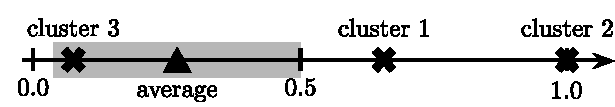
\includegraphics[width=0.6\textwidth]{images/cluster_labeling_2.pdf}
	\caption{Cluster labelling method 2: The distance of each cluster to the overall average blog posts is calculated. If the distance is below or over a certain threshold (shaded in grey), the cluster obtains a label. In this example a label is assigned to cluster 1 and 2.}
	\label{fig:cluster_labeling_2}
\end{figure}


\paragraph{Method 3}
As with method 2, we calculate the difference to the average for each cluster and feature.
However, we also normalize them to the total range this feature has for our data.
Then, we pick the $n$ most significant of these differences for each cluster and use them to label it.
Significance, in this case, is mostly determined by how great the deviation from the average is: The larger the deviation the higher the significance.
The only exception to this is that being very close to to the average is considered slightly more significant than only being fairly close to it.

In our example, clusters 2 and 3 would most likely get the label ``longest'' or ``shortest blog posts'' respectively.
Cluster 1 on the other hand would be eligible for the low significance label ``average length blog posts'' but might not get it if it has $n$ more significant labels.
With this method, every cluster is guaranteed to get a set number of labels, even if it has no features that deviate from the average.


%!TEX root = ../paper.tex

\subsection{Classification}
\label{sec:classification}



After we cluster all blog posts, e.g. in a database, we need a way to deal with new blog posts which are added at a later point.
Optimally, we want a new blog post to be sorted into the cluster it would have also landed in if it were part of the original clustering.
To ensure this outcome, we could add the new blog post to the data set and then run the whole clustering again on all documents.
However this seems inefficient because of the potentially huge number of documents which would have to be clustered again, compared to the fact that we want to assign a cluster to only one new blog post.
Furthermore we do not want the addition of one blog post to change the cluster assignments of other blog posts, which could happen if the clustering step was repeated.


Instead, we use a separate classification step to find a suitable cluster assignment.
For this, we first extract the same set of features from the new blog post that were previously extracted before the clustering of all posts.
Then, we use the results from the clustering step, the feature vectors of the clustered blog posts and their cluster assignments, to determine the best match for the new blog post.
To this end, we used machine learning techniques which are explained in Section~\ref{sec:impl_classification} in detail.


%!TEX root = ../paper.tex

\section{Implementation}
\label{sec:implementation}
\begin{itemize}
	\item Give use some insights into the algorithm
	\item Point out major technical challenges
\end{itemize}


%!TEX root = ../paper.tex

\subsection{Data Source}
\label{sec:data_source}

The main data source we used was the Spinn3r Data Set [TODO: reference], which contains data from about 65 million blog posts.
These blog posts come in various different languages and only sparse metadata.
Many of them do not have an author attributed which makes them unusable for testing our algorithm's performance.
Even those blog posts which have some author data, only have their username with no way of telling whether that alias is used by multiple authors in the database and thus might also provide faulty results.
Additionally, due to originating from different blogging websites, the blogs' content had very different formatting: Some of them still contained html tags while some others had their line breaks removed, rendering all features relying on them obsolete [TODO: leave this sentence in?].
Thus, we concluded that the Spinn3r Data Set, while still being a target data set for running our program on, was useless for testing its performance and determining which techniques work best.


Hence, we manually created our own, small data set, consisting of 15 blog posts for each of six German blogs, for a total of 90 blog posts.
This small test set provided us with a gold standard for all our future tests and allowed us to run multiple, performance intensive tests in a realistic time frame.
\subsection{Features}
\label{sec:features}

An individual's writing style can be discerned by various attributes or features inherent to any written text.
Some of these features are topic-dependent, e.g. the count of occurrence for each existing word in the ``Bag of Words'' model [TODO: Reference?].
A text containing an above average number of occurrences of words like ``DNA'', ``sequence'', ``genome'', and ``mutation'' will most likely be from the field of genome research.
Thus, this feature will be similar for most texts from this domain and therefore is topic-dependent.


However, since we want to classify blog posts independent of topic, we can only utilize topic-independent features.
We represent these features as real valued numbers, normalized to be between 0 and 1.
Each attribute of a text can be represented by multiple features, for example the frequency of punctuation characters can have one feature per punctuation character, denoting that character's frequency as a fraction of all characters.
After calculating all features, the combination of them is interpreted as a vector for each text and then passed on to the machine learning or classification step.


We have selected a number of these topic-independent features from~\cite{madigan2005author} and added a few of our own, which are more tailored towards blog posts, e.g. emoticons.
A list of the feature types we initially used can be found in Table~\ref{tab:featureTable} along with their respective individual feature count.


One of the features we utilized, the FunctionWord feature might appear to clash with our desire to create a topic-independent algorithm which does not use a Bag of Words model.
However, function words are words with little or no lexical meaning, mainly used to create the grammatical structure of a sentence. [TODO: Reference?]
Thus, they are actually topic-independent and the frequency of their usage has been successfully utilized to identify authors \cite{mosteller1962applied}.
We also tried to achieve topic-independence for our list of common abbreviations which we used in the same way.


Our emoticon feature is one that we selected to specifically target the blogging realm.
Since emoticons hardly ever appear in traditional written works, they have not been utilized when trying to identify authors outside of the internet.
In the blogosphere, however, there are some users who utilize lots of emoticons and others that don't use them at all.
The types of emoticons used also differ from person to person which is why we decided to implement that feature as a binary value of a certain emoticon appearing in the text or not.
%[TODO: If we need to fill room: Explain some features in detail (vocabulary richness, PoS tags)]


After evaluating our features (see Section~\ref{sec:evaluation_clustering}) we decided to drop the Prefix/Suffix feature and keep all others.

\begin{table}[h]
    \begin{center}
    \begin{tabular}{p{2.6cm}|p{8.2cm}|p{1.2cm}}
    Feature					& Description																	& Count				\\ \hline
    BlankLine				& 1 divided by number of Blank Lines in the text								& 1					\\ \hline
    CapitalLetter			& Capital letters divided by all letters										& 1					\\ \hline
    Emoticon				& Boolean value for occurrence of known emoticons								& 9					\\ \hline
    FunctionWord			& Fraction of words that are a known function word. [TODO: List in appendix?]	& 280[DE] 280[EN]	\\ \hline
    Abbreviations			& Words that are a known abbreviation [TODO: List in appendix?]					& 53[DE] 53[EN]		\\ \hline
    NumberCharacter			& Fraction of characters that are numeric characters (0-9)						& 1					\\ \hline
    Paragraph				& Number of Paragraphs divided by average Paragraph								& 1					\\ \hline
    PoSTag					& Fraction of words that have a certain Part-of-Speech Tag~\cite{toutanova2000enriching}                                                                                                        & 55[DE] 46[EN]  	\\ \hline
    PostLength				& 1 divided by the number of characters											& 1					\\ \hline
    PrefixSuffix			& 2-letter Prefixes/Suffixes divided by total number of Prefixes/Suffixes		& 676 			 	\\ \hline
    Punctuation Character	& Fraction of characters that are a known punctuation character [TODO: List in appendix?]
                                                                                                            & 11				\\ \hline
    SentenceLength			& 1 divided by the average sentence length										& 1 				\\ \hline
    singleOccurring Word	& Words that only occur once divided by all distinct words						& 1					\\ \hline
    UpperCaseWord			& Words that are fully in upper case divided by all words						& 1					\\ \hline
    WordFrequency			& 1 divided by the average number of occurrences per word						& 1					\\ \hline
    WordLength				& 1 divided by the average word length											& 1					\\
    \end{tabular}
    \end{center}
	\caption{Feature Table. Implemented features with descriptions and the count of individual features they contribute to the feature vector.}
	\label{tab:featureTable}
\end{table}

%!TEX root = ../paper.tex

\subsection{Clustering}
\label{sec:clustering}

After extracting all features and vectorizing them for each blog post in the database, we group them into clusters according to the similarity of their feature vectors.
To this end, we use a k-means algorithm which is a method from vector quantization.
Afterwards the resulting clusters are labelled, so that the user knows what kind of blog posts he can expect in a specific cluster.

\subsubsection{K-Means Algorithm}
\label{sec:k-means}
K-means creates $k$ clusters from $n$ vectors by randomly selecting $k$ points from the vector space as cluster centroids.
Then, each vector or point is assigned to its nearest cluster centroid according to its Euclidean distance to those centroids.
Afterwards, the cluster centroids are repositioned to the center of all vectors/points which were assigned to them.
These last two steps are repeated until the cluster centroids converge.
The resulting assignment of the vectors (and thus their corresponding blog posts) to the clusters is the same as the final assignment performed by the k-means algorithm.
For our implementation we used the k-means algorithm offered my Mahout\footnote{\url{https://mahout.apache.org/}}, which can be executed efficiently among a cluster with a large amount of data~\cite{esteves2011k}.

To run a k-means algorithm, the value $k$ has to be set beforehand.
$K$ represents the number of clusters and thus the number of similar writing styles, which should be determined.
Finding an appropriate value for $k$ depends highly on the use case.
One use case could be to find exact authors, so that one cluster, i.e. writing style group, would correspond to one author.
One cluster would only contain blog posts of one author.
The value $k$ should therefore be similar to the number of expected authors.
Another use case could be to find similar writing style groups.
One cluster would then contain blog posts from multiple authors having a similar writing style.
In this case $k$ should be chosen much lower than the actual number of authors.

% [TODO: Graphic?]
% [TODO: discuss other algorithms?]

\subsubsection{Cluster Labelling}
\label{sec:cluster_labeling}
Labelling the resulting clusters helps the user to distinguish between them.
The labels indicate what kind of blog posts are in those clusters, so that the user gets an idea what to expect from blog posts in this cluster.

The current research in the field of cluster labelling focuses on topic-dependent labels.
Because we want to cluster by writing style rather than topic, we were unable to use those techniques.
Howver, trying to find universally accepted writing styles leads to labels like ``informative'' or ``opinion piece'', which merely represent the text's intention, not the author's personal style. [TODO: reference].
Thus, these types of labels were also not applicable for our use case.

Therefore, we implemented our own cluster labelling methods, which consider the most important features of a cluster.
These methods are explained using the following example:
The current feature is ``length of blog posts'' and we have three clusters with the following values for the current feature:
\begin{center}
\begin{tabular}{c|c|c}
  Cluster 1 & Cluster 2 & Cluster 3 \\ \hline
  0.7 & 1 & 0.1 \\
 \end{tabular}
\end{center}
\paragraph{Method 1}
For each feature and cluster, the highest and lowest value is determined.
Those clusters are then labelled with appropriate labels.

In the example cluster 2 has the highest value and gets the label ``longest blog posts''.
The label ``shortest blog posts'' is assigned to cluster 3, because this cluster has the lowest value.
Using this method only the most significant labels are set.
But a cluster may not obtain any label when it does not have any extreme features.

\paragraph{Method 2}
First, the average vector of all blog posts is calculated.
In a second step, the distance for each feature and cluster to that average vector is determined.
If the distance is over a certain threshold, the cluster is labelled.

The example is shown in Figure~\ref{cluster_labeling_2}.
Because cluster 3 is not over the threshold, thus the length of the blog post is not significant for the cluster, no label is assigned to that cluster.
Cluster 1 and 2 are both over the threshold and obtain the label ``long blog posts''.
This method assigns more labels to clusters than method 1, but can also lead to clusters without any labels if all of a cluster's feature have average values.

\begin{figure}[ht]
	\centering
	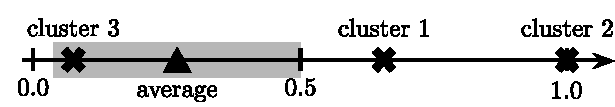
\includegraphics[width=0.33\textwidth]{images/cluster_labeling_2.pdf}
	\caption{}
	\label{cluster_labeling_2}
\end{figure}

\paragraph{Method 3}
As with Method 2, we calculate the difference to the average for each cluster and feature.
However, we also normalize them to the total range this feature has for our data.
Then, we pick the $n$ most significant of these differences for each cluster and use them to label it.
Significance, in this case, is mostly determined by how great the deviation from the average is: The larger the deviation the higher the significance.
The only exception to this is that being very close to to the average is considered slightly more significant than only being fairly close to it.

In our example, Clusters 2 and 3 would most likely get the label ``longest'' or ``shortest blog posts'' respectively.
Cluster 1 on the other hand would be eligible for the low significance label ``average length blog posts'' but might not get it if it has $n$ more significant labels.
With this method, every cluster is guaranteed to get a set number of labels, even if it has no features that deviate from the average.

%!TEX root = ../paper.tex

\subsection{Classification}
\label{sec:classification}

After we came up with clusters and cluster labels for all blog posts in a database, we need a method to classify new blog posts. % e.g. so new clustering is not needed for every single blog post
To achieve this we calculate the same features vectors for the single new blog post, as were extracted for the blog posts in the original clustering.
Based on these feature vectors we can now decide to which cluster the blog post belongs.


The first naive idea that came into our mind was to calculate the euclidean distance from the blog post to the center points of the clusters.
The resulting cluster would then be the one with the lowest distance.
While this method is computationally simple and fast, it might not provide the best possible results.
Therefore we looked at more sophisticated approaches that were used for similar problems before.
We applied two of those methods, k-Nearest Neighbor algorithm and a Support Vector Machine [TODO: references?].


\subsubsection{k-Nearest Neighbor}
\label{sec:k_nearest_neighbor}


The k-Nearest Neighbor algorithm selects the number of $k$ vectors which are closest to the feature vector of the new blog post.
Then it returns the cluster that is most common amongst these neighbors as a result. 
For example consider the scenario depicted in Fig.~\ref{fig:naive}.
The naive method of calculating the euclidean distance between the cluster center and the feature vector of the new blog post would have cluster 1 as a result.
However the k-Nearest Neighbor algorithm with, for example $k=5$, returns cluster 2, because 4 out of the 5 closest neighbors belong to cluster 2.
This also seems correct compared to our human intuition, because the feature vector of the new blog post seems to be naturally belonging to cluster two.


\begin{figure}
    \centering
    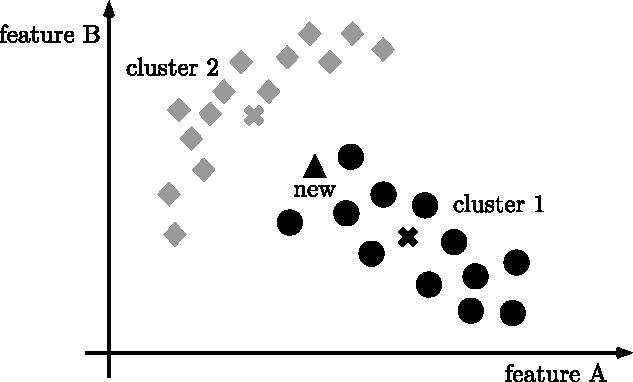
\includegraphics[]{images/naive.pdf}
    \caption{The naive approach, which calculates the euclidean distance to the center of the cluster, would put the new blog post into cluster 1. The k-Nearest Neighbor algorithm would return cluster 2 as a result.}
    \label{fig:naive}
\end{figure}


\subsubsection{Support Vector Machine}
\label{sec:support_vector_machine}


A Support Vector Machine creates a model to distinguish between the different clusters by calculating borders between the clusters.
These borders can be thought of as functions in the same vector space as the feature vectors.
If the Support Vector Machine uses a linear model, this might look like Fig.~\ref{fig:svm}, represented in a two-dimensional graph.
Both the dotted and the dashed line serve as examples for a possible border, but the Support Vector Machine should usually tend to use the model with more distance to all feature vectors.
In this case the dashed line would more accurately divide cluster 1 and 2.


\begin{figure}
    \centering
    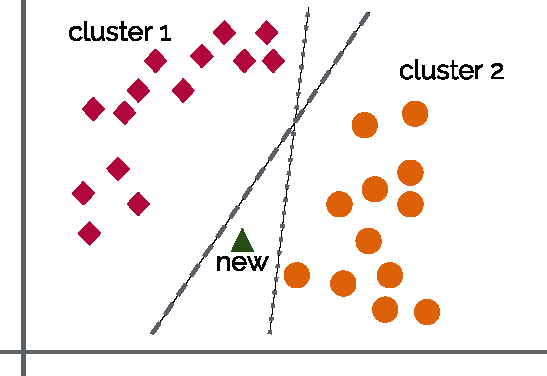
\includegraphics[]{images/svm.pdf}
    \caption{Two differently configured Support Vector Machines might provide the two different lines as borders between the different clusters. The dotted line would result in the blog post belonging to cluster 1, while the dashed line would return cluster 2 as a result.}
    \label{fig:svm}
\end{figure}


%!TEX root = ../paper.tex
\section{Evaluation and Results}
\label{sec:results}


To evaluate our two separate steps, we need a suitable data set with certain characteristics.
Firstly we want to measure the performance of our clustering into similar author groups.
Based on how this performance changes, when adding or removing features, we can also evaluate the value gain of features.
After we have the results from the clustering, we then use this mapping of blog posts on clusters to evaluate the prediction of new blog posts.
For example the cluster a blog post belongs to in the clustering result, is also the one we want to identify the blog post as, if it was not part of the clustering and classified afterwards.


%!TEX root = ../paper.tex

\subsection{Data Sources}
\label{sec:data_sources}


The data source should contain only blog posts written in one language and blog posts having author metadata attributed to them.
With the help of the author information we can evaluate our system under the assumption that one author has the same writing style over a series of blog posts they wrote.

Because we could not find such an open, free data source, we manually created our own small data set.
This data set consists of 15 blog posts for each of six German blogs, for a total of 90 blog posts.
This small test set provided us with a gold standard for all our future tests and allowed us to run multiple, performance intensive tests in a feasible time frame.

After evaluating and improving our system with our small data set, we ran it with the 2011 Spinn3r data set\footnote{\url{http://www.icwsm.org/data/}}, which contains data from about 65 million blog posts.
These blog posts come in various different languages and only with sparse metadata.
Many of them do not have an author attribute, which makes them unusable for testing our algorithm's performance.
%Even those blog posts which have some author data, only have their username with no way of telling whether that alias is used by multiple authors in the database and thus might also provide faulty results.
%Additionally, due to originating from different blogging websites, the blogs' content had very different formatting: Some of them still contained html tags while some others had their line breaks removed, rendering all features relying on them obsolete.
%Thus, we concluded that the Spinn3r data set, while still being a target data set for running our program on, was useless for testing its performance and determining which techniques work best.





\subsection{Evaluation of Clustering}
\label{sec:evaluation_clustering}
To evaluate our \textit{k-means} algorithm we evaluated the feasibility and usefulness of our features (see Table~\ref{tab:featureTable}) by splitting them into 12 semantically related groups and then ran our \textit{k-means} clustering algorithm on each of the $2^{12} = 4096$ possible permutations of active features using our small test data set (see Section~\ref{sec:data_sources}).
We set the number of desired clusters to six, allowing for the possibility of each author getting their own cluster.
We then used this scenario as a gold standard and calculated precision, recall and F-measure wrt. an author as shown here:
\begin{equation}
	Precision = \frac{TP}{TP + FP} \\
	\label{eq:precision}
\end{equation}
\begin{equation}
	Recall = \frac{TP}{TP + FN} \\
	\label{eq:recall}
\end{equation}
\begin{equation}
	F-measure = \frac{2 \times Recall \times Precision}{Recall + Precision}
	\label{eq:fMeasure}
\end{equation}
For each author we find the cluster, which contains the highest number of documents from that author, the dominant cluster.
We assume that this is the best matching cluster for the author, so all documents from that author should belong to that cluster.
Based on this assumption, if author A has the dominant cluster C, we then define $TP$, $FP$ and $FN$ in the following way:
\begin{itemize}
	\item[$TP$:] Number of blog posts of author A, which are assigned to cluster C. \\
	\item[$FP$:] Number of blog posts from other authors, which are assigned to cluster C. \\
	\item[$FN$:] Number of blog posts of author A, which are not assigned to cluster C.
\end{itemize}

From these 4096 individual test runs we selected some meaningful data points to base our conclusions on.
One of these meaningful feature combinations was the one that gave the best overall F-measure of $61.62\%$.
This feature combination did not contain the \textit{prefix/suffix} and the \textit{part-of-speech tag} features.
This was surprising for us, because~\cite{madigan2005author} listed these as some of the features that performed best for them and because our own tests showed that only having these features active on their own provided us with better results than only having one of the other features turned on.
Looking further into the data, we found that turning off the \textit{prefix/suffix} or the \textit{part-of-speech tag} feature while all other features remained active provided us with better results than having all features active at a time (see Table~\ref{tab:feature_evaluation_1}).

\begin{table}[ht!]
	\begin{center}
    \begin{tabular}{l|r|r}
	Feature name		& F-measure without & Difference to all features \\ \hline \hline
	All features active	& 0.4152833313 & $\pm$0.0 \\ \hline \hline
	Emoticon			& 0.3757936508 & +0.0438422688 \\ \hline
	Blank line			& 0.4074074074 & +0.0078759239 \\ \hline
	Post length			& 0.4196359196 & +0.0043525883 \\ \hline
	Word frequency		& 0.4130983959 & +0.0021849354 \\ \hline
	Upper case			& 0.4144100548 & +0.0008732765 \\ \hline
	Capital letter		& 0.4148865024 & +0.0003968289 \\ \hline
	Function word		& 0.4150935674 & +0.0001897639 \\ \hline
	Character frequency	& 0.4151904736 & +0.0000928577 \\ \hline
	Word length			& 0.4152373925 & +0.0000459388 \\ \hline
	Sentence length		& 0.4152833313 & $\pm$0.0 	   \\ \hline
	Part-of-speech tag				& 0.4196359196 & -0.0043525883 \\ \hline
	Prefix/suffix		& 0.4712048408 & -0.0559215095 \\
    \end{tabular}
    \end{center}
	\caption{The F-measure having all features but one active and the difference to the F-measure having all features active. Having the \textit{part-of-speech tag} feature or the \textit{prefix/suffix} feature active, decreases the overall F-measure.}
	\label{tab:feature_evaluation_1}
\end{table}

We concluded that the \textit{prefix/suffix} and \textit{part-of-speech tag} features provided merely decent (but not great) results on their own.
Due to their high number of individual features, we can use them alone quite well to distinguish blog posts, however the overall quality is not as good as other single features combined.
Features with only one individual value might provide a clearer separation but only in a single dimension.
This means that they are not good for creating a larger number of clusters, which is what would have been required for a good performance in our test with only one active feature.
However, due to the clear separation they provide, adding more small features (and thus dimensions) drastically improves the test results.
If we then add in the high dimensional but only mediocre features such as \textit{prefix/suffix} and \textit{part-of-speech tag} as well, the test results become worse because the positive impact of the low dimensional features is lessened by the sheer amount of dimensions added to the feature vector.
Thus, their good performance is being overshadowed by the high dimensional features' mediocrity.


Ultimately, we decided not to use the \textit{prefix/suffix} and \textit{part-of-speech tag} features, since they both lowered performance significantly.
Dropping them both meant that the number of features we had in a vector was now only a fraction of the previous amount, which gave our small but well-performing features much more impact.


The resulting F-measure for our \textit{k-means} algorithm when having all but the \textit{prefix/suffix} and \textit{part-of-speech tag} feature enabled is $61.64\%$.
When looking at the individual blog posts' classification, we noticed that the blog posts of two authors would mostly be sorted into the same cluster due to their feature vectors being quite similar.
We concluded that these two authors actually had a similar writing style and that this meant that the F-measure could not become much better due to our gold standard assuming one cluster per author.


\subsection{Evaluation of Classification}
\label{sec:evaluation_classification}

For evaluating our classification methods we used ten-fold cross validation~\cite{kohavi1995study}.
We divide our test data set into ten sets, each set containing nine blog posts.
Then we train our classification algorithms on nine of these ten sets and use the last set for testing.
This process is repeated ten times, so each one of these sets was a test set once.
Each time the precision is calculated and at the end the overall average precision is determined.


Training the \textit{support vector machine} means that a new model based on the training data set is created.
This model is then used for determining a cluster for each blog posts in the test set.
The \textit{k-nearest neighbor} algorithm uses the training data set as known data points (see Section~\ref{sec:k_nearest_neighbor}).


After finding the optimal parameters for both methods, we achieved $97.77\%$ precision for \textit{k-nearest neighbor} and $98.89\%$ precision for our \textit{support vector machine} in the ten-fold cross validation.


Thus, our result of $\sim60\%$ F-measure for clustering appears to be a lot better than those from related work in this field.
This is mainly due to the different problem domain though:
We merely try to find similar writing style groups, while most of the related work tried to identify the exact author to a document.
Since this problem is harder than ours, simply because the solution space is a lot larger, results that appear worse at first glance (such as the $20\%$ accuracy of Narayanan et al.~\cite{narayanan2012feasibility}) are to be expected.
On the other hand, Koppel et al.~\cite{koppel2003automatically}, who try to correctly identify an author's gender by their writing style, achieve a precision of over $80\%$ since this problem is smaller than even our six assumed writing styles.
The fact that our results lie somewhere between these two other approaches to (respectively) more and less difficult problems is thus exactly what was to be expected.

%!TEX root = ../paper.tex

\section{Related Work}
\label{sec:related}
\begin{itemize}
	\item Who inspired your work?
	\item Which aspect do you improve?
	\item What are the basic foundations?
\end{itemize}

%!TEX root = ../paper.tex
\section{Conclusion and Future Work}
\label{sec:conclusion}

Nowadays, everyone can write a blog posts fairly easy.
Thus, the amount of blog posts and authors increases quickly, making the task of identifying an exact author nearly impossible.
In this paper, we presented an approach of dividing a set of blog posts into different groups, each group representing an individual writing style and therefore similar authors.
Thus, we are reducing the potential candidates by an order of magnitude or more and we can aid the user in getting much closer to the correct author.


For our approach multiple features for identifying different writing styles were tested and evaluated.
Having a feature, which results in hundreds of subfeatures by having only a few other features, adulterated the results immensly.
A k-means algorithm is used to cluster the blog posts based on the selected features.
An evaluation on a small test data set showed that our k-means algorithm has an f-measure of $61.64\%$.
To determine a cluster, i.e. writing style, of a new blog posts, different classification methods were examained.
It was shown, that k-nearest neighbor performed slighty better ($97.77\%$) than a support vector machine ($91.86\%$).


Our approach performs very well for the use case of finding blog posts similar to ones a user already likes.
Since we can do so across topics, a new type of recommendation engine could be employed to recommend blogs based on writing style alone.
Our system could be employed by blogging websites to increase traffic and thus advertising revenue by recommending interesting blogs.


Our program’s results and its usability could be improved in various ways: Adding more languages to our program’s repertoire would greatly increase its scope.
This would merely require adjusting the calculation of some of the features by adding an appropriate Part-of-Speech tagger and a function word list as well as new tests on the performance and feasibility of each feature.


Utilizing a larger and more diverse data set with a proper gold standard could allow for improved evaluation of our program’s ability to find exact matches for unknown authors.
This would also allow for a more in-depth discussion of which additional features to use and how to weight them.


Additional work could also be put into our clustering step by adding an additional phase prior to the k-means algorithm to attempt to find the optimal number of clusters for it to use.
Alternatively, evaluating the feasibility of other clustering algorithms is also an option.

\newpage
\bibliographystyle{abbrv}
\bibliography{references}

\end{document}